\chapter{Baseline Motion System} \label{chap:motion}
    This chapter covers the systems governing the baseline motion of the robot, meaning the motion over simple flat terrain. 
    First the kinematics of the robot are defined, next the walking gait state machine is
    described, and finally the equations to defining a foots path of motion is described. An overview of these systems can be seen in figure \ref{fig:motion_system}.
    \begin{figure}[h]
        \centering
        % \hspace{-1.38cm}
        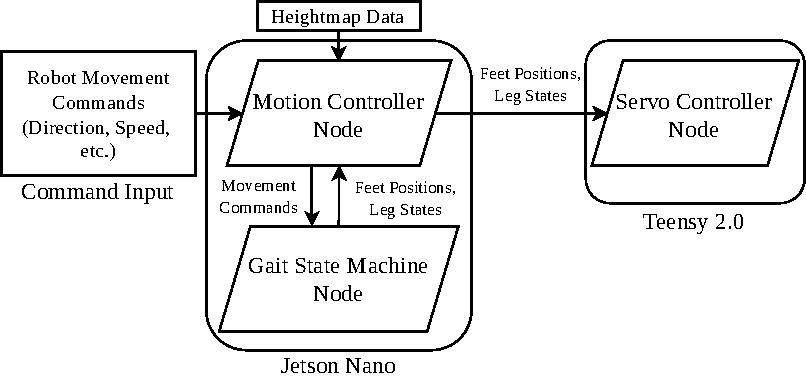
\includegraphics{Diagrams-MotionSystem.drawio.pdf}
        \caption{Motion System Overview}
        \label{fig:motion_system}
    \end{figure}
    \section{Overview}
        % This chapter describes the systems governing the motion of the robot, such as leg motion planning and gait generation.
        The basic operation of the motion system is as follows, first the robot is commanded to walk in a certain direction, at a
        certain speed and body height. These commands are sent from the base station to Jetson Nano on the robot,
        the motion controller node on the Jetson Nano then sends these commands to the gait state machine node, at a fixed frequency.
        The gait state machine uses the received direction stride length to generate leg states (swinging or supporting) and the ideal
        final position of each foot. These states and positions are sent back to the motion controller node where the positions are adjusted
        based on the heightmap data to ensure stable footing. The leg states and adjusted feet positions are then sent to the servo 
        controller node, this node controls the servos to move the robots feet to their final positions, either in a arc or linearly,
        depending on their state (swinging or supporting). %A high level diagram of the motion system can be seen in \ref{fig:motion_system}.

    \section{Kinematics}
        When commanding a foot position, the servo controller requires a function to calculate servo angles. While the foot arc planner, see section 
        \ref{sec:arc_generation}, requires the current position of the feet to function. The \ac{ik} and \ac{fk} functions described in this section provide
        this functionality. 
        
        \subsection{Coordinate Frames}
            The coordinate frames relevant to the kinematics of the robot are the body coordinate frame, \fbody, and the leg frame, \fleg. All foot targets/positions are specified
            if the body coordinate frame, while the kinematic systems operate in the leg coordinate frame. Thus a conversion from the body to leg frames is required. 
            Figure \ref{fig:coords_top} show the world, body and multiple leg coordinate frames.
            \begin{figure}[h]
                \centering
                % \hspace{-1.38cm}
                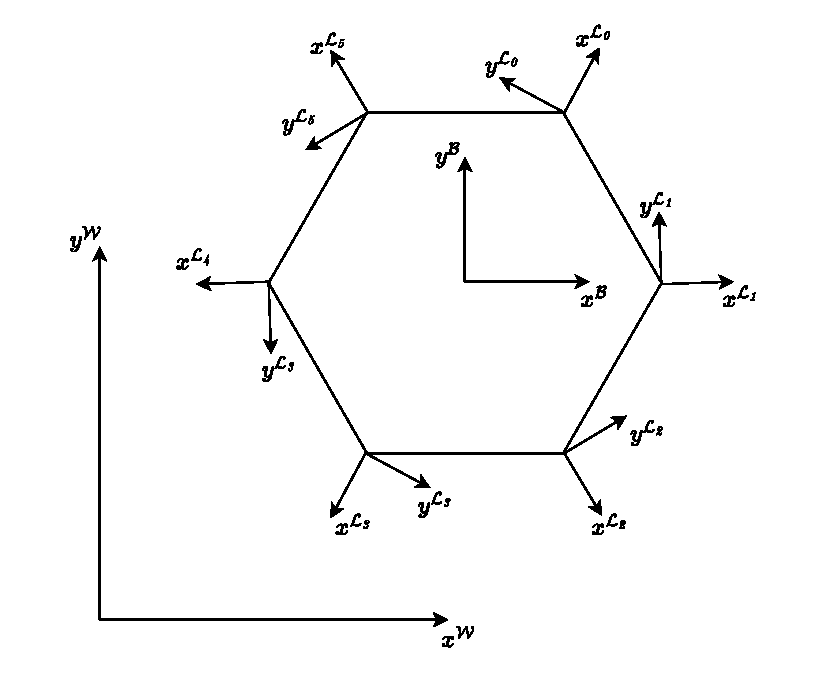
\includegraphics[width=.7\textwidth]{Diagrams-BodyFrame.drawio.pdf}
                \caption{World, body and leg coordinate frames.}
                \label{fig:coords_top}
            \end{figure}

            \noindent
            The leg coordinate systems are simply rotated and shifted from the body coordinate system. This transformation,\transframe{\bm{x}^\fbody}{\fbody}{\fleg} is defined by equation \ref{eq:body_to_leg},
            further explained explained in appendix \ref{app:transforms}.
            \begin{equation}\label{eq:body_to_leg}
            \begin{split}
                \bm{x}^\fleg &= \transframe{\bm{x}^\fbody}{\fbody}{\fleg} \\
                & = \bm{Q}_i^\fbody\cdot\bm{x}^\fbody\cdot\bm{Q}^{\fbody^{-1}}_{i} - \bm{R}_i
            \end{split}
            \end{equation}

            \noindent
            where the \(\fleg\) is the coordinate frame of leg \(i\), \(\bm{Q}_i^\fbody\) is the rotation of said coordinate frame and \(\bm{R}^\fbody_i\) is the root position of
            said leg coordinate frame in the body coordinate frame. For more detail on this transformation, such as the values of \(\bm{Q}_i^\fbody\) and \(\bm{R}^\fbody_i\), please see
            appendix \ref{app:transforms}.

            Now that positions can be transformed into the leg coordinate frame the kinematic equations, as described in the following sections, can be applied. The kinematic equations are defined
            with reference to the variables in the leg frame as shown in figure \ref{fig:kinematics}.
            \begin{figure}[h]
                \centering
                % \hspace{-1.38cm}
                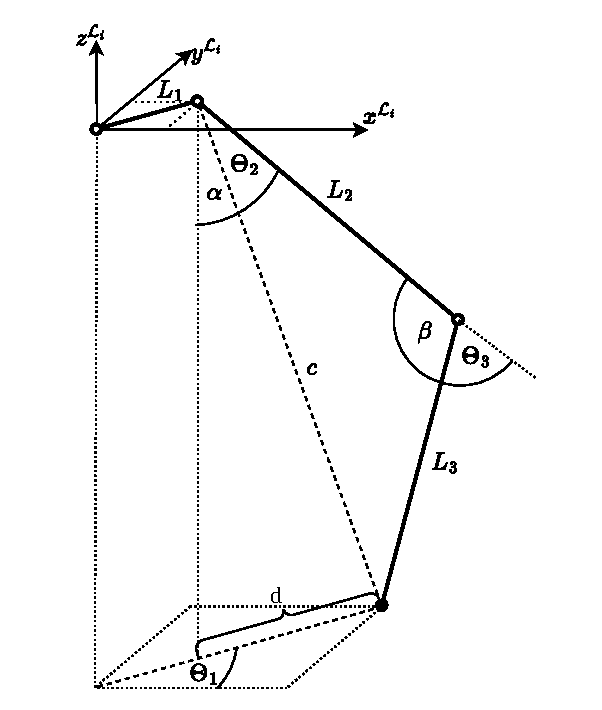
\includegraphics[clip, trim=0 0 1.1cm 0]{Diagrams-Kinematics.drawio.pdf}
                \caption{Leg coordinate frame with kinematic variables.}
                \label{fig:kinematics}
            \end{figure}

        \newpage
        \subsection{\acf{ik}}
            The \ac{ik} function calculates the leg servo angles, \(\bm{\Theta} = [\Theta_1, \Theta_2, \Theta_3]^T_{\displaystyle ,}\) required
            to move the foot to the given target position vector, \(\bm{t} = [x_t,y_t,z_t]^T_{\displaystyle .}\)
            \hbox{Equation \ref{eq:ik}} describes the \ac{ik} function.
            \begin{equation}\label{eq:ik}
                \bm{\Theta}(x_t,y_t,z_t) =
                                    % \begin{bmatrix}
                                    %     \Theta_1\\
                                    %     \Theta_2\\
                                    %     \Theta_3
                                    % \end{bmatrix}
                                    % =
                                    \begin{bmatrix}
                                        \arctan{\left(\dfrac{x_t}{y_t}\right)}\\[0.5cm]
                                        \dfrac{\pi}{4} - \alpha - \arctan{\left(\dfrac{y_t}{d-L_1}\right)}\\[0.5cm]
                                        \dfrac{\pi}{2} - \beta
                                    \end{bmatrix}
            \end{equation}
            where \(\alpha\), \(\beta\), \(c\) and \(d\) are calculate as shown in equations \ref{eq:alpha} to \ref{eq:dik}. For derivations of these variable
            please see \ref{app:kinematic}.
            \begin{align}
                \alpha &= \arcsin{\left(\frac{L_3\sin{\beta}}{c}\right)} \label{eq:alpha} \\[0.5cm]
                \beta &= \arccos{\left(\dfrac{L_1^2 + L_2^2 -c^2}{2L_1L_2}\right)}\\[0.5cm]
                c &= \sqrt{(d-L_1)^2+z_t^2}\\[0.5cm]
                d &= \sqrt{x_t^2 + y_t^2} \label{eq:dik}
            \end{align}
        \subsection{\acf{fk}}
            The \ac{fk} function calculates the position vector of a foot, \(\bm{p}_f = [x_f,y_f,z_f]^T\),
            given the current angles of the leg servos, \(\bm{\theta} = [\theta_1, \theta_2, \theta_3]^T\).
            \begin{align}
                \bm{p}_f(\theta_1,\theta_2,\theta_3) =
                                % \begin{bmatrix}
                                %     x_c\\
                                %     y_c\\
                                %     z_c
                                % \end{bmatrix}
                                % =
                                \begin{bmatrix}
                                    d\cos{\theta_1}\\
                                    d\sin{\theta_1}\\
                                    L_2\sin{\theta_2} + L_3\sin{\left(\theta_2 + \theta_3\right)}
                                \end{bmatrix}
            \end{align}
            where \(d\) is calculated as shown in in equation \ref{eq:dfk}.
            \begin{equation}\label{eq:dfk}
                d = L1 + L_2\sin{\theta_2} + L_3\sin{(\theta_2 + \theta_3)}
            \end{equation}
        
        \newpage
        \subsection{Angular Rate} \label{sec:ang_rate}
            To move a foot on a desired path it is important to not only know the absolute angle of the three leg servos, but also the angular rates of all three
            servos. If the servos are all moved at the same rate, the shape of the path that the foot follows will not be linear, but rather dependant on the
            current foot position. This is undesirable, thus equations \ref{eq:rate} define the derivative of the \ac{ik} equations (\ref{eq:ik}), i.e. the angular
            rate, given the target movement speeds of a foot, \(\dot{x}\), \(\dot{y}\) and \(\dot{z}\).

            \begin{equation}\label{eq:rate}
                \bm{\omega}(\dot{x}, \dot{y}, \dot{z}) =
                                    % \begin{bmatrix}
                                    %     \omega_1\\
                                    %     \omega_2\\
                                    %     \omega_3
                                    % \end{bmatrix}
                                    % =
                                    \begin{bmatrix}
                                        \dfrac{- x\dot{y} + y \dot{x}}{x^2 + y^2}\\[0.5cm]
                                        \dfrac{\left[(L_1 - d)\dot{z} + z\dot{d}\right]\alpha + \Big[(L_1 - d)^2 + z^2\Big]\arctan{\left(\dfrac{L_1-d}{z}\right)}\dot{\alpha}}{(L_1 - d)^2 + z^2}\\[0.8cm]
                                        -\dot{\beta} 
                                    \end{bmatrix}
            \end{equation}
            where \(\dot\alpha\), \(\dot\beta\), \(\dot{c}\) and \(\dot{d}\) as shown in equations \ref{eq:alphadot} to \ref{eq:cdot}.
            \begin{align}
                \dot{\alpha} &= \frac{ L_3\left[ c\cos(\beta)\dot{\beta} - \sin(\beta)\dot{c} \right] }{ c^2\sqrt{-\dfrac{L_3^2\sin^2(\beta)}{c^2}+1} } \label{eq:alphadot} \\[0.5cm] 
                \dot{\beta} &= \frac{ 2c\dot{c} }{ L_2L_3\sqrt{4 - \dfrac{(L_2^2+L_3^2-c^2)^2}{L_2^2L_3^2}} } \label{eq:betadot} \\[0.5cm]
                \dot{c} &= \frac{-(L_1 - d)\dot{d} + z\dot{z}}{\sqrt{(L_1 - d)^2 + z^2}} \label{eq:bdot} \\[0.5cm]
                \dot{d} &= \frac{x\dot{x} + y\dot{y}}{\sqrt{x^2 + y^2}} \label{eq:cdot}
            \end{align}
    
    \newpage
    \section{Walking Gait}
        To move the hexapod must support its body with some of its legs while the remaining legs swing towards their new targets,
        at which point the swinging legs become the new supporting. The sequence in which the legs support and swing is called the walking gait.
        Figure \ref{fig:gait_patterns} shows three different gait patterns that can be used with a hexapod, the wave ripple and tripod gait \citep{Darbha2017AnOS}.
        The dark cell represents a swinging leg and the light cell a supporting leg.
        \begin{figure}[h]
            \centering
            % \hspace{-1.38cm}
            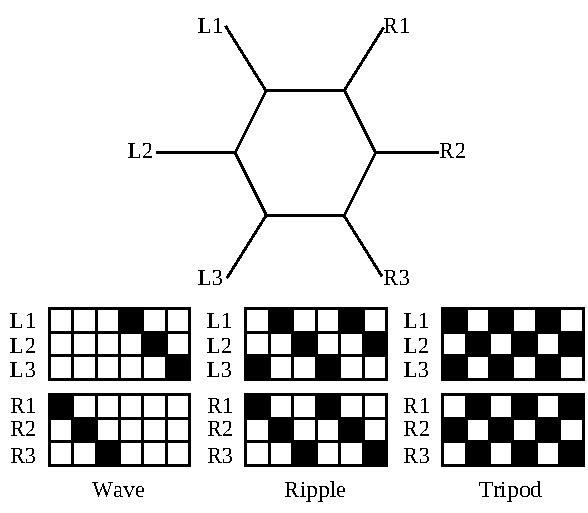
\includegraphics{Diagrams-GaitDiagram.drawio.pdf}
            \caption{Three hexapod gait patterns.}
            \label{fig:gait_patterns}
        \end{figure}

        \noindent
        The wave gait moves one leg at a time while supporting with the remaining 5, the ripple gait moves two legs at a time, and the tripod moves
        three legs at a time.

        The speed of the hexapod is based on the parameters of the gait, specifically as described in equation \ref{eq:speed},
        \begin{equation} \label{eq:speed}
            v = \frac{S}{D\tau}
        \end{equation}
        where \(S\) is the stride length, \(tau\) is the gait period and \(D\) is the duty factor. \(D\) is defined as the time a leg is in the support phase relative to its swing phase.
        The wave, ripple and tripod gaits have a duty factor of \(\frac{5}{6}\), \(\frac{2}{3}\) and \(\frac{1}{2}\) respectively.
        
        From this it is clear that the wave gait is the slowest while the tripod gait is the fastest, and the ripple gait is in between.
        It should however be noted the gait's stability is inverse to their speed.

        The gait that will be used in this system is the tripod gait, which is the most common gait for hexapods as it supports with three legs, while maximising speed. Even though this is less stable than
        the wave and ripple gaits, it does maintain natural stability with three contact points, which is adequate for most circumstances.

        \subsection{Stride Reference Frame}
            When describing the stride of the robot it is important to note which reference frame is being used. Figure \ref{fig:stride_body} shows
            the stride of a tripod gait in the body reference frame, \(\fbody\).
            \begin{figure}[h]
                \centering
                % \hspace{-1.38cm}
                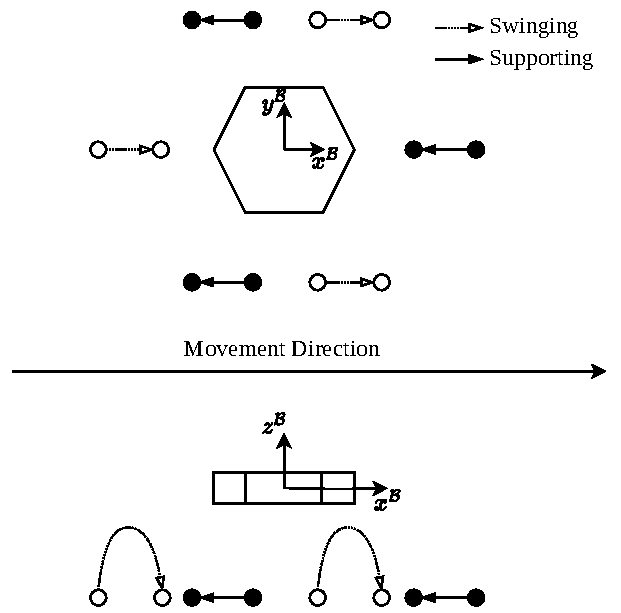
\includegraphics{Diagrams-StrideDiagramLocal.drawio.pdf}
                \caption{Hexapod stride relative to body coordinates.}
                \label{fig:stride_body}
            \end{figure}

            \noindent
            As can be seen, the swinging legs move in the direction of movement, following a arced path.
            While the supporting legs move in the opposite direction of movement following a linear path. 

            \newpage
            \noindent
            However, when looking at the same stride in the world reference frame, \(\fworld\), as can be seen in figure \ref{fig:stride_world},
            the supporting legs appear to stay stationary, while the swinging legs move double the distance relative to that in the body reference frame.
            \begin{figure}[h]
                \centering
                % \hspace{-1.38cm}
                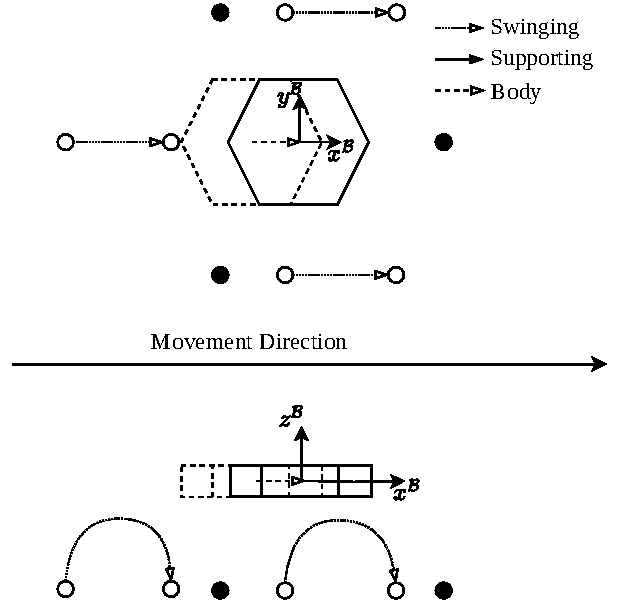
\includegraphics{Diagrams-StrideDiagramGlobal.drawio.pdf}
                \caption{Hexapod stride relative to world coordinates.}
                \label{fig:stride_world}
            \end{figure}

            \noindent
            This is important to note because, as further discussed in section \ref{sec:choosing_nominal}, the nominal foot positions are chosen in the body reference frame, but must target a
            position in the world reference frame.
        
        \newpage
        \subsection{State Machine}
            The state machine used to realise the tripod gait used in the robot is quite simple, comprised of only two states, stepping and
            resting, as can be seen from figure \ref{fig:gaitSM}. Table \ref{tab:state_defs} defines the actions that should be taken during
            each state.

            The primary computation done by this state machine is calculating which legs are supporting and which are swinging, which occurs
            on entering the "Stepping" state. This function is described in section \ref{sec:supp_swing_calc}.

            \begin{figure}[h]
                \centering
                % \hspace{-1.38cm}
                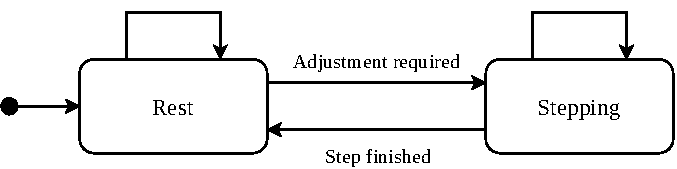
\includegraphics{Diagrams-GaitSM.drawio.pdf}
                \caption{Gait State Machine}
                \label{fig:gaitSM}
            \end{figure}

            \begin{table}[h]
                \center
                \begin{tabularx}{\textwidth}{|l|X|}
                    \hline
                    \multicolumn{2}{|c|}{Rest State Definition} \\
                    \hline
                    Enter Condition & Has all feet reached their targets? \\
                    \hline
                    On Entering & Set all leg states as supporting. \\
                    \hline
                    While Active & Do nothing \\
                    \hline
                \end{tabularx}
                
                \bigskip
                \noindent
                \begin{tabularx}{\textwidth}{|l|X|}
                    \hline
                    \multicolumn{2}{|c|}{Stepping State Definition} \\
                    \hline
                    Enter Condition & Is there a mismatch between feet targets and current position? \\
                    \hline
                    On Entering & Calculate and set the leg states based on walking direction, see section \ref{sec:supp_swing_calc}. Choose and optimise nominal targets
                    for the current step, see chapter \ref{chap:optimisation}\\
                    \hline
                    While Active & Adjust feet targets based on direction, stride length and robot height, see chapter \ref{chap:optimisation}\\
                    \hline
                \end{tabularx}
                \caption{State Definitions}
                \label{tab:state_defs}
            \end{table}

        \newpage
        \subsection{Choosing The Supporting And Swinging Legs} \label{sec:supp_swing_calc}
            The robot body is divided up into sextants, centered around the nominal leg positions. When calculating
            the swinging legs it is first determined in which sextant the movement direction vector falls, this is called the active sextant.
            The leg related with the active sextant, and the two opposite, are then chosen as swinging, with the remaining three legs chosen as supporting.
            The states of the legs are encapsulated by the boolean array, \(\bm{S_i}\), defined by equation \ref{eq:is_swing},
            where a 1 indicates swinging and 0 supporting.
            \begin{equation}\label{eq:is_swing}
                \bm{S}_{\bm{i} - \xi}=[i \text{ is even}]
            \end{equation}
            where \(\xi \in i\) is the active sextant/leg number, and,
            \[i = \seq{0}{1}{5}\]

            Figure \ref{fig:sextants} illustrates and example with sextant 1 being active. Thus legs 1, 3 and 5 are swinging, while legs 0, 2 and 4 are supporting.
            \begin{figure}[h]
                \centering
                \hspace{1.1cm}
                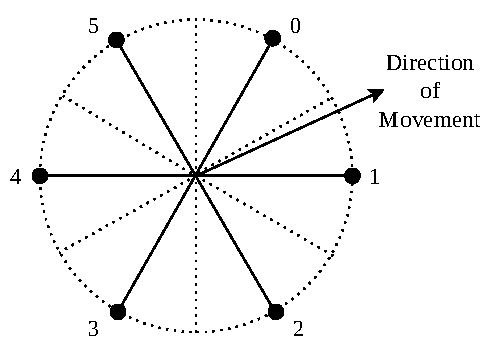
\includegraphics[clip, trim=0 0.25cm 0 0.25cm]{Diagrams-Sextants.drawio.pdf}
                \caption{Leg sextants, with sextant 1 being active.} 
                \label{fig:sextants}
            \end{figure}
            
            \noindent
            This of course would not be sufficient to define a walking gait, as at the end of each step \(\bm{S_i}\) does not invert.
            Thus and additional step after equation \ref{eq:is_swing} is added. The current horizontal length of leg \(\xi\), defined as \(l_\xi\), is compared to its nominal
            horizontal length, \(L_\xi\). If \(l_\xi\ > L_\xi\), invert \(\bm{S_i}\). As shown in equation \ref{eq:negate_is_swing}.
            \begin{equation} \label{eq:negate_is_swing}
                \bm{S}_{\bm{i} - \xi} =
                                                    \begin{cases}
                                                        \bm{i} \setminus \bm{S}_{\bm{i} - \xi} & l_\xi > L_\xi \\
                                                        \bm{S}_{\bm{i} - \xi} & l_\xi \leq L_\xi
                                                    \end{cases}\\[0.1cm]
            \end{equation}

            \newpage
        \subsection{Choosing nominal foot positions}\label{sec:choosing_nominal} 
            Once the active and inactive legs have been selected it is required to choose nominal targets for all the feet. Sections \ref{sec:support} and \ref{sec:swing}
            describe the process for finding the support and swinging leg targets; It should be noted that target matrices, denoted by \(\bm{t}\), are common between these two sections, but are computed
            differently depending on whether the leg is swinging or supporting.
                
            \subsubsection{For Supporting Legs} \label{sec:support}
                The supporing leg nominal trargets are chosen with using equations \ref{eq:move_vec} and \ref{eq:opt_supp}, with reference
                to figure \ref{fig:supp_targ}.
                \begin{figure}[h]
                    \centering
                    % \hspace{1.1cm}
                    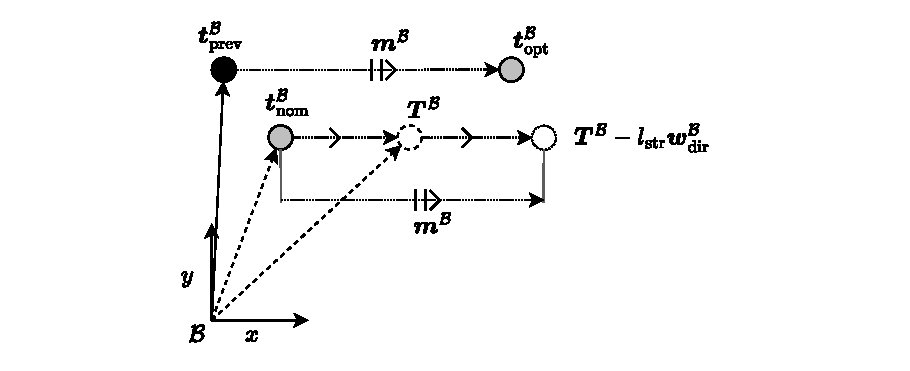
\includegraphics[clip, trim=3cm 0.25cm 3.4cm 0.25cm]{Diagrams-ChooseNominalSupp.drawio.pdf}
                    \caption{Supporting target choosing diagram} 
                    \label{fig:supp_targ}
                \end{figure}

                \noindent
                First the required move vectors, \(\bm{m} ^\fbody\), are calculated in equation \ref{eq:move_vec},
                \begin{equation}\label{eq:move_vec}
                    \mdim{\boldsymbol{m}^\fbody}{3}{1} =  (\bm{T}^\fbody - l_\text{str} \bm{\bm{w}_\text{dir}}^\fbody) - \bm{t_\text{nom}}^\fbody
                \end{equation}
                where \(\bm{T}^\fbody\) contains the constant rest positions the feet, \(l_\text{str}\) is the desired stride length, \(\bm{w}_\text{dir}^\fbody\)
                contains the desired walk directions, and \(\bm{t}_\text{nom} ^\fbody\) contains the nominal targets as calculated in
                equation \ref{eq:swing_nom}.

                Then the optimised targets, \(\bm{t_\text{opt}} ^\fbody\), are calculated as the addition of the previous targets and the move vector in equation \ref{eq:move_vec},
                \begin{equation} \label{eq:opt_supp}
                    \mdim{\boldsymbol{t}_\text{opt}^\fbody}{3}{6} = \bm{t}_\text{prv}^\fbody + \bm{m}^\fbody
                \end{equation}
                where \(\bm{t}_\text{prv}^\fbody\) contains the previous, optimised, targets. Note that equation \ref{eq:opt_supp} does not include the optimisation
                function \textcolor{red}{XXXX}, this is because the supporting feet will not move relative to the terrain, and thus do not need optimising.

            \newpage
            \subsubsection{For Swinging Legs} \label{sec:swing}
                The swinging leg nominal targets are chosen with reference to figure \ref{fig:swinging_targ}.
                \begin{figure}[h]
                    \centering
                    % \hspace{1.1cm}
                    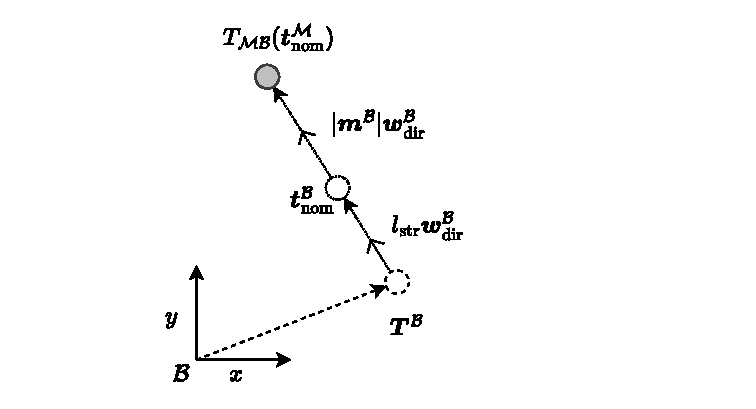
\includegraphics[clip, trim=3.25cm 0.25cm 4.9cm 0.3cm]{Diagrams-ChooseNominalSwing.drawio.pdf}
                    \caption{Swinging target choosing diagram} 
                    \label{fig:swinging_targ}
                \end{figure}

                \noindent
                The nominal targets in map space, \(\bm{t_\text{nom}} ^{\fmap}\), are calculated as in equation \ref{eq:t_map},
                \begin{equation} \label{eq:t_map}
                    \mdim{\boldsymbol{t}_\text{nom}^{\fmap}}{3}{6} = \transframe{\bm{T}^\fbody + \left(l_\text{str}+|\bm{m}^\fbody|\right)\bm{w}_{dir}^\fbody}{\fbody}{\fmap}
                \end{equation}
                where \(\bm{T}^\fbody\) contains the constant rest positions the feet, \(l_\text{str}\) is the desired stride length, \(\bm{w}_\text{dir}^\fbody\)
                contains the desired walk directions. \(\avg\bm{m}^\fbody\) is the average move vector 

                For use in equation \ref{eq:move_vec}, the swinging legs nominal targets, \(\bm{t_\text{nom}} ^\fbody\), are calculated as 
                in equation \ref{eq:swing_nom},
                \begin{equation} \label{eq:swing_nom}
                    \mdim{\boldsymbol{t}_\text{nom}^\fbody}{3}{6} = \bm{T}^\fbody + l_{str}\bm{w}_\text{dir}^\fbody
                \end{equation}

                Note that \(\transframe{\bm{t}_\text{nom}^{\fmap}}{M}{L}\) is quite similar to \(\bm{t}_\text{nom}^\fbody\), the difference is that \(\bm{t}_\text{nom}^{\fmap}\) is set such that it
                will align with \(\bm{t}_\text{nom}^\fbody\)
                at the end of the step. Thus, the omission of the average supporting move vector, \(\avg \bm{m}^\fbody\), in calculating \(\bm{t}_\text{nom}^\fbody\)
                in equation \ref{eq:swing_nom}.
                Meaning at until the end of the step \(\bm{t}_\text{nom}\inrefframe{M}\) and \(\bm{t}_\text{nom}^\fbody\) will point 
                to different positions if world space. This is due to needing to account for body movement in world space, but not in local space.

        \newpage
    \section{Foot Motion} \label{sec:arc_generation}
        When taking a step the foot can not simply be moved to its destination in a straight line, as doing so will cause the foot to be dragged on the terrain,
        impeding the movement of the robot. Thus it is required to move the foot in an arc like motion to clear any obstacles that might be in its path.


        \subsection{Existing System}
            The existing system will, at the start of each step, compute an arc for each foot to follow, this arc is then sent to the servo controller
            to be executed. The arc is computed as a polynomial passing through three points, the initial point\(q_i\), the middle point \(q_m\), and the final point \(q_f\).
            Figure \ref{fig:old_arc_vars} shows the variables used to calculate this arc.
            \begin{figure}[h]
                \centering
                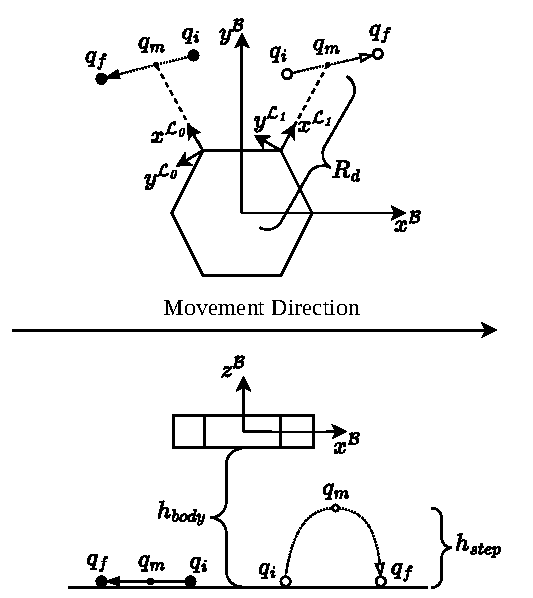
\includegraphics{Diagrams-ArcCalc.drawio.pdf}
                \caption{Variables for calculating foor arc.}
                \label{fig:old_arc_vars}
            \end{figure}

            % \noindent
            % Equation \ref{eq:old_arc} shows the calculations used to find the starting, middle and end points shown in figure \ref{fig:old_arc_vars}.

            % \begin{align}\label{eq:old_arc}
            %     OldArcEquation\\
            %     OldArcEquation\\
            %     OldArcEquation\\
            %     OldArcEquation\\
            %     OldArcEquation\\
            %     OldArcEquation\\
            %     OldArcEquation\\
            %     OldArcEquation\\
            %     OldArcEquation
            % \end{align}
            % where etc\dots

            \newpage
            \noindent
            While efficient and effective in ideal conditions, this method of defining the arc has poor performance when considering external
            influences. If for example the robot has to adjust the final target of its feet mid step, this arc would have to be recomputed in its entirety,
            thus leading to possible performance concerns.

            In addition to this Text, the current system is designed with the assumption that the starting position of the foot is grounded, thus if the arc is recomputed
            mid step the arc will be undesirable, as it will rise with the desired step height for a second time. This is illustrated in Figure \ref{fig:old_arc}.

            \begin{figure}[h]
                \centering
                \hspace{-1.38cm}
                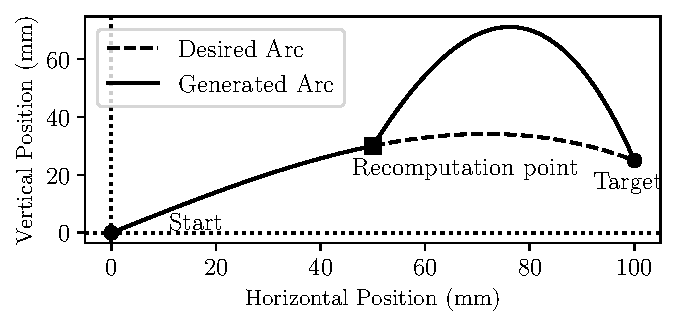
\includegraphics[clip, trim=0 0.25cm 0 0.25cm]{old_path.pdf}
                \caption{Existing arc recomputation problem}
                \label{fig:old_arc}
            \end{figure}

        \newpage
        \subsection{Improved System}
            The improved system solves this problem by utilising a flow function. During a step, this function will continuously calculate the
            direction that the foot must move to reach its destination. Thus this system is resilient to external disturbances and is capable of adjusting to
            varying destination and step height requirements. 
            
            The flow field is designed to first move the foot vertically upwards until horizontal coplanar with the destination, and then to follow a
            arc to the destination with a defined step height, this can be adjusted to make the arc start before or after coplanar. The step height can be adjusted at any point in time and the flow field will adjust accordingly.
            Figure \ref{fig:foot_arc} illustrates the field function and is described in section \ref{sec:flow_function}.
            \begin{figure}[h]
                \centering
                \hspace{-1.38cm}
                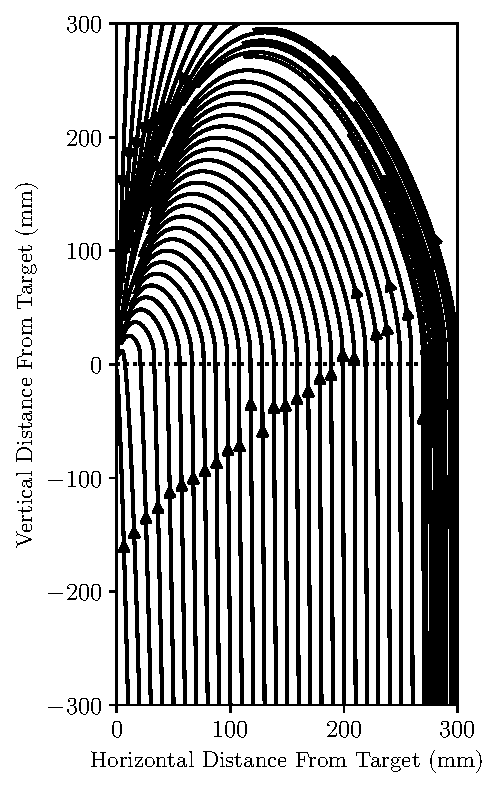
\includegraphics[clip, trim=0 0.25cm 0 0.25cm]{foot_path.pdf}
                \caption{End effector movement path}
                \label{fig:foot_arc}
            \end{figure}

            \subsubsection{Flow Function Description} \label{sec:flow_function}
                The flow function, \(\rho(x,y)\), uses the gradient function of a parabola passing through the point \([0,0]\) and \([x,y]\) as a basis, where point \([x,y]\)
                is the current point that is being evaluated and \(x\) is the horizontal distance between the destination and the current point and \(y\) the
                vertical distance. The final function is described by equations \ref{eq:rho} to \ref{eq:sigmoid}, for the process of designing the flow function
                please see appendix \ref{app:flow_function}.
                \begin{equation} \label{eq:rho}
                    \begin{aligned}
                        \rho(x,y) &= \frac{\delta}{\delta x\delta y}&&f_a(x,y)x^2 + f_b(x,y)x + C\\
                        &= &&2f_a'(x,y)x + f_b'(x,y)    
                    \end{aligned}
                \end{equation}
                where, %\(f_a'(x,y)\) and \(f_b'(x,y)\) are defined as follows:
                \begin{align} \label{eq:fa}
                    f_a'(x,y) &= -\left|\frac{v_h}{x}\right| - \left|S(y)\right|\\
                    f_b'(x,y) &= \frac{y}{x} - f_a(x,y)
                \end{align}
                with \(v_h\) being the variable describing the step height and \(S(y)\) being a sigmoid like function 
                responsible for the initial vertical rise. \(S(y)\) is defined in Equation \ref{eq:sigmoid}.
                \begin{equation} \label{eq:sigmoid}
                    S(y) = \frac{0.515(y-q)}{1+\left|y-q\right|-0.505}
                \end{equation}
                where \(q\) is the variable that determines at which vertical displacement the leg path transitions from primarily an vertical motion to
                an arc motion. Figure \ref{fig:sigmoid_like} illustrates the sigmoid like function for different values of \(q\).
                \begin{figure}[h]
                    \centering
                    \hspace{-1.38cm}
                    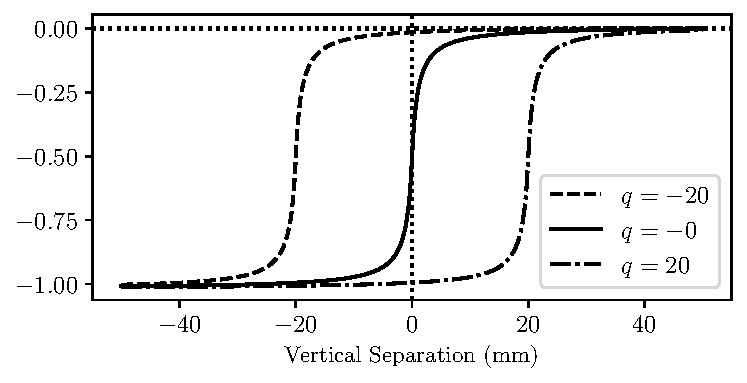
\includegraphics[clip, trim=0 0.25cm 0 0.25cm]{sigmoid_like.pdf}
                    \caption{Sigmoid Like}
                    \label{fig:sigmoid_like}
                \end{figure}

                \noindent
                Note that the 0.515 and 0.505 values in equation \ref{eq:sigmoid} are set to make its output range from roughly -1 to 0 over the active range.
